%package list
\documentclass{article}
\usepackage[top=3cm, bottom=3cm, outer=3cm, inner=3cm]{geometry}
\usepackage{multicol}
\usepackage{graphicx}
\usepackage{url}
%\usepackage{cite}
\usepackage{hyperref}
\usepackage{array}
%\usepackage{multicol}
\newcolumntype{x}[1]{>{\centering\arraybackslash\hspace{0pt}}p{#1}}
\usepackage{natbib}
\usepackage{pdfpages}
\usepackage{multirow}
\usepackage[normalem]{ulem}
\useunder{\uline}{\ul}{}
\usepackage{svg}
\usepackage{xcolor}
\usepackage{listings}
\lstdefinestyle{ascii-tree}{
	literate={├}{|}1 {─}{--}1 {└}{+}1 
}
\lstset{basicstyle=\ttfamily,
	showstringspaces=false,
	commentstyle=\color{red},
	keywordstyle=\color{blue}
}
%\usepackage{booktabs}
\usepackage{caption}
\usepackage{subcaption}
\usepackage{float}
\usepackage{array}

\newcolumntype{M}[1]{>{\centering\arraybackslash}m{#1}}
\newcolumntype{N}{@{}m{0pt}@{}}


%%%%%%%%%%%%%%%%%%%%%%%%%%%%%%%%%%%%%%%%%%%%%%%%%%%%%%%%%%%%%%%%%%%%%%%%%%%%
%%%%%%%%%%%%%%%%%%%%%%%%%%%%%%%%%%%%%%%%%%%%%%%%%%%%%%%%%%%%%%%%%%%%%%%%%%%%
\newcommand{\itemEmail}{jchuraaca@unsa.edu.pe}
\newcommand{\itemStudent}{Julio Rubén Chura Acabana}
\newcommand{\itemCourse}{ F. de Programción 2}
\newcommand{\itemCourseCode}{20230472}
\newcommand{\itemSemester}{I}
\newcommand{\itemUniversity}{Universidad Nacional de San Agustín de Arequipa}
\newcommand{\itemFaculty}{Facultad de Ingeniería de Producción y Servicios}
\newcommand{\itemDepartment}{Departamento Académico de Ingeniería de Sistemas e Informática}
\newcommand{\itemSchool}{Escuela Profesional de Ingeniería de Sistemas}
\newcommand{\itemAcademic}{2023 - B}
\newcommand{\itemInput}{Del 22 de Enero 2023}
\newcommand{\itemOutput}{Al 29 de Enero 2023}
\newcommand{\itemPracticeNumber}{23}
\newcommand{\itemTheme}{Proyecto Final}
%%%%%%%%%%%%%%%%%%%%%%%%%%%%%%%%%%%%%%%%%%%%%%%%%%%%%%%%%%%%%%%%%%%%%%%%%%%%
%%%%%%%%%%%%%%%%%%%%%%%%%%%%%%%%%%%%%%%%%%%%%%%%%%%%%%%%%%%%%%%%%%%%%%%%%%%%

\usepackage[english,spanish]{babel}
\usepackage[utf8]{inputenc}
\AtBeginDocument{\selectlanguage{spanish}}
\renewcommand{\figurename}{Figura}
\renewcommand{\refname}{Referencias}
\renewcommand{\tablename}{Tabla} %esto no funciona cuando se usa babel
\AtBeginDocument{%
	\renewcommand\tablename{Tabla}
}

\usepackage{fancyhdr}
\pagestyle{fancy}
\fancyhf{}
\setlength{\headheight}{30pt}
\renewcommand{\headrulewidth}{1pt}
\renewcommand{\footrulewidth}{1pt}
\fancyhead[L]{\raisebox{-0.2\height}{
\includegraphics[width=3cm]{img/logo_episunsa.png}}}
\fancyhead[C]{\fontsize{7}{7}\selectfont	\itemUniversity \\ \itemFaculty \\ \itemDepartment \\ \itemSchool \\ \textbf{\itemCourse}}
\fancyhead[R]{\raisebox{-0.2\height}{
\includegraphics[width=1.2cm]{img/logo_abet}}}
\fancyfoot[L]{Estudiante Julio Rubén Chura Acabana}
\fancyfoot[C]{\itemCourse}
\fancyfoot[R]{Página \thepage}

% para el codigo fuente
\usepackage{listings}
\usepackage{color, colortbl}
\definecolor{dkgreen}{rgb}{0,0.6,0}
\definecolor{gray}{rgb}{0.5,0.5,0.5}
\definecolor{mauve}{rgb}{0.58,0,0.82}
\definecolor{codebackground}{rgb}{0.95, 0.95, 0.92}
\definecolor{tablebackground}{rgb}{0.8, 0, 0}

\lstset{frame=tb,
	language=bash,
	aboveskip=3mm,
	belowskip=3mm,
	showstringspaces=false,
	columns=flexible,
	basicstyle={\small\ttfamily},
	numbers=none,
	numberstyle=\tiny\color{gray},
	keywordstyle=\color{blue},
	commentstyle=\color{dkgreen},
	stringstyle=\color{mauve},
	breaklines=true,
	breakatwhitespace=true,
	tabsize=3,
	backgroundcolor= \color{codebackground},
}

\begin{document}
	
	\vspace*{10px}
	
	\begin{center}	
		\fontsize{17}{17} \textbf{ Informe de Laboratorio \itemPracticeNumber}
	\end{center}
	\centerline{\textbf{\Large Tema: \itemTheme}}
	%\vspace*{0.5cm}	
	
	\begin{flushright}
		\begin{tabular}{|M{2.5cm}|N|}
			\hline 
			\rowcolor{tablebackground}
			\color{white} \textbf{Nota}  \\
			\hline 
			\\[30pt]
			\hline 			
		\end{tabular}
	\end{flushright}	
	
	\begin{table}[H]
		\begin{tabular}{|x{4.7cm}|x{4.8cm}|x{4.8cm}|}
			\hline 
			\rowcolor{tablebackground}
			\color{white} \textbf{Estudiante} & \color{white}\textbf{Escuela}  & \color{white}\textbf{Asignatura}   \\
			\hline 
			{\itemStudent \par \itemEmail} & \itemSchool & {\itemCourse \par Semestre: \itemSemester \par Código: \itemCourseCode}     \\
			\hline 			
		\end{tabular}
	\end{table}		
	
	\begin{table}[H]
		\begin{tabular}{|x{4.7cm}|x{4.8cm}|x{4.8cm}|}
			\hline 
			\rowcolor{tablebackground}
			\color{white}\textbf{Laboratorio} & \color{white}\textbf{Tema}  & \color{white}\textbf{Duración}   \\
			\hline 
			\itemPracticeNumber & \itemTheme & 04 horas   \\
			\hline 
		\end{tabular}
	\end{table}
	
	\begin{table}[H]
		\begin{tabular}{|x{4.7cm}|x{4.8cm}|x{4.8cm}|}
			\hline 
			\rowcolor{tablebackground}
			\color{white}\textbf{Semestre académico} & \color{white}\textbf{Fecha de inicio}  & \color{white}\textbf{Fecha de entrega}   \\
			\hline 
			\itemAcademic & \itemInput &  \itemOutput  \\
			\hline 
		\end{tabular}
	\end{table}
	
	\section{Tarea}
	\begin{itemize}		
		\item Cree una versión del videojuego de estrategia usando componentes básicos GUI: Etiquetas, botones,
		cuadros de texto, JOptionPane, Color.
	\end{itemize}
	
	\section{Equipos, materiales y temas utilizados}
	\begin{itemize}
		\item Sistema Operativo Windows
		\item Apache NetBeans IDE 19
		\item OpenJDK 64-Bits 20.0.2.
		\item Git 2.42.0.
		\item Xampp v3.3.0
		\item Cuenta en GitHub con el correo institucional.
		\item Base de Datos e interfaz gráfica de usuario
	\end{itemize}
	
	\section{URL de Repositorio Github}
	\begin{itemize}
		\item URL del Repositorio GitHub para clonar o recuperar.
		\item \url{https://github.com/JulioChura/fp2-23b.git}
		\item URL para el laboratorio 01 en el Repositorio GitHub.
		\item \url{https://github.com/JulioChura/fp2-23b/tree/main/fase03/lab23_juegoFinal}
	\end{itemize}
	
	\section{Actividades con el repositorio GitHub}
	
	
	
	
	
	
	
	\subsection{Preparación del espacio de trabajo}
	
	\begin{lstlisting}[language=bash,caption={Se crea un nuevo proecto en Netbeans }][H]
		mkdir lab23_juegoFinal
		xcopy C:\Users\USUARIO\Desktop\fp2-23b\fase02\lab22 C:\Users\USUARIO\Desktop\fp2-23b\fase02\lab23_juegoFinal /s /e
		cd ..\lab23
	\end{lstlisting}
	
	
	\subsection{Estructura básica de las Ventanas}
	
	\begin{figure}[H]
		\centering
		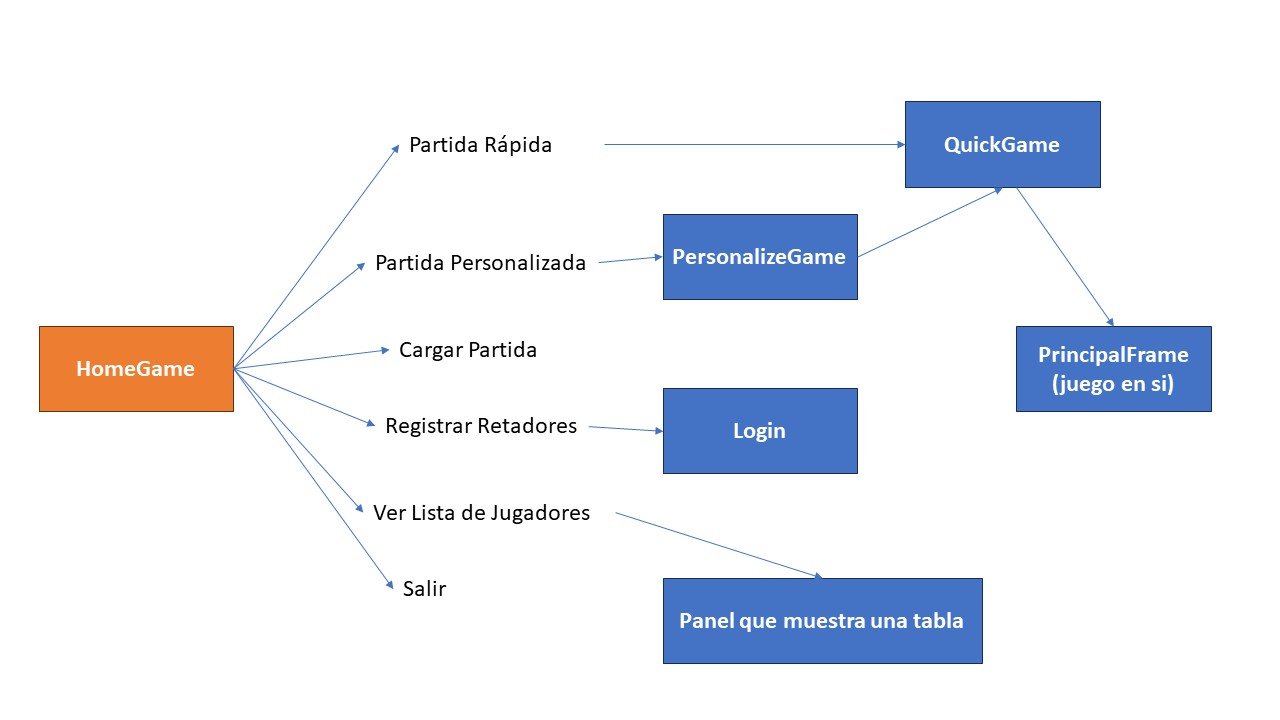
\includegraphics[width=1\textwidth,keepaspectratio]{img/estructura.jpg}
		%\includesvg{img/automata.svg}
		%\label{img:mot2}
		%\caption{Product backlog.}
	\end{figure}
	
	
	

	
	\subsection{Evolución del código y test del mismo}
	
	
	\begin{lstlisting}[language=bash,caption={Commit: de0f855ead9602d62a573015aa8941d54e373d59 }][H]
		git add Menu.java
		git commit -m "Debido a la dificultad de trabajar, se decide mudar los archivos del proyecto a netbeans, hasta este cambio se creo un metodo dentro de conectar para crear un nuevo usuario"			
		git push -u origin main
	\end{lstlisting}
	
	\begin{itemize}	
	\item Debido a que este trabajo requería el uso  de interfaz gráfica, se opta de mudar el proyecto de vs code a Netbeans debido a su herramienta que tiene para poder crear GUI de forma más sencilla y personalizables. También ya se estaba viendo para conectarse a una de datos, por lo que se se copia la clase Conectar.java de un trabajo que se dejó en los grupos de teoría. Esta clase que nos permite conectarnos con la bae de datos que tiene implementado el patrón de diseño Singleton. Además en el proyecto se decide crear paquetes que permiten diferenciar las clases que serán GUI, las clases que manejan la lógica y la que nos permitirá usar base de datos (persistencia)
	\end{itemize}
	
	
	\begin{figure}[H]
		\centering
		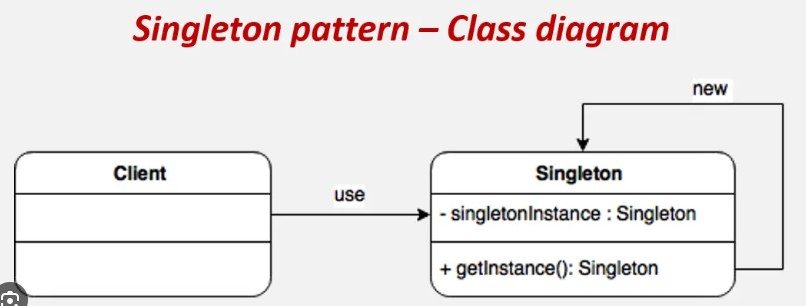
\includegraphics[width=1\textwidth,keepaspectratio]{img/singleton.jpg}
		%\includesvg{img/automata.svg}
		%\label{img:mot2}
		%\caption{Product backlog.}
	\end{figure}

	\begin{itemize}	
		\item Este es el diagrama del patrón de diseño en mención
	\end{itemize}
	
	
		\begin{figure}[H]
		\centering
		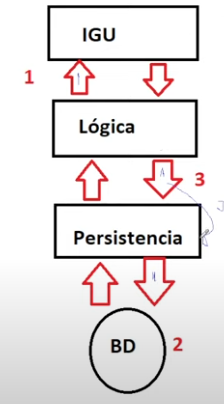
\includegraphics[width=0.5\textwidth,keepaspectratio]{img/modelo.png}
		%\includesvg{img/automata.svg}
		%\label{img:mot2}
		%\caption{Product backlog.}
	\end{figure}
	
	\begin{itemize}	
		\item Para el proyecto se trató de aplicar este modelo
	\end{itemize}

	
	
	\begin{lstlisting}[language=bash,caption={Commit: 8b752b0993f8facea77c5b3a97a7856e0e6e73ed }][H]
		git add .
		git commit -m "Se completa la logica para poder registrar nuevos jugadores"			
		git push -u origin main
	\end{lstlisting}
	
	\begin{itemize}	
	\item En esta parte se crea la ventana para que el usuario pueda logearse. Tiene un diseño sencillo.
	\end{itemize}
	
		\begin{figure}[H]
		\centering
		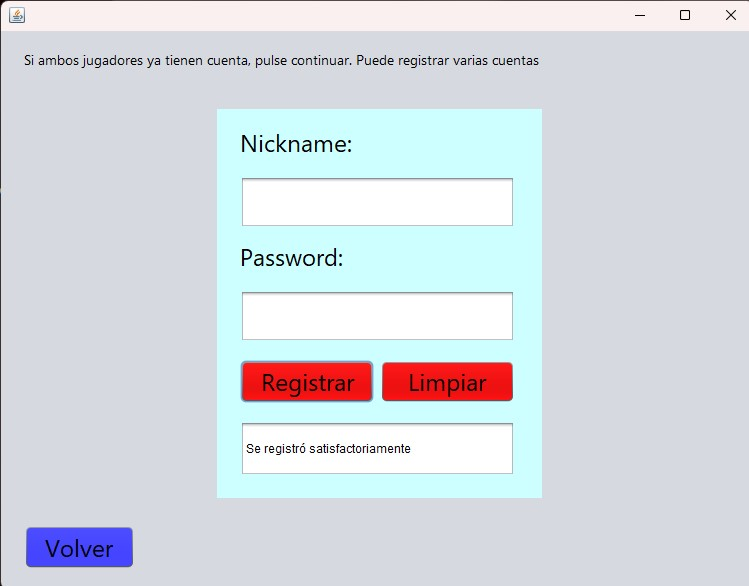
\includegraphics[width=1\textwidth,keepaspectratio]{img/login.jpg}
		%\includesvg{img/automata.svg}
		%\label{img:mot2}
		%\caption{Product backlog.}
	\end{figure}
	
	\begin{itemize}	
		\item Este vendría a ser el diseño final. El usuario podrá ver si se registró en el área de texto. Como se puede apreciar se acaba de registrar un nuevo usuario
	\end{itemize}
	
	
	
	\begin{lstlisting}[language=bash,caption={Commit: ad82e8abf5a8c58897d2ac6b10c4959f81e56965 }][H]
		git add .
		git commit -m "En login ya se crean las demas tablas y para ello se modifica la clase Conectarr"			
		git push -u origin main
	\end{lstlisting}
	
	
	\begin{itemize}
	\item Ya que se ha implementado en la interfaz gráfica del logeo, ahora toca crear en la clase Conectar un método que nos permita realizar una consulta a la basey verificar si el usuario en mención ya tiene una cuenta o no, como este es el primer commit para esta vesión del método, adelanto que también se incorporará la función de poder crear las tablas partidas y ejércitos 
	\end{itemize}
	
	
	
	\begin{lstlisting}[language=bash,caption={Commit: 962b10dee42f6ec69b35431ea5b3b76094dbd215 }][H]
		git add .
		git commit -m "Se modifica la clase Conectar la cual ahora tiene un metodo para obtener las victorias, ademas se hacen leves cambios en la clase para hacer las consultas"			
		git push -u origin main
	\end{lstlisting}
	
	
	\begin{itemize}
	\item Ya en la parte cuando nos registramos para poder jugar, se tenía pensado crear el objeto Jugador para que guarde los atributos de la tabla jugadores, esto para más adelante incorporar funciones como cargar partida, sin embargo, por falta de tiempo la idea se descarta, por lo que la conusulta para obtener la racha de victorias es algo innecesario. 
	\end{itemize}
	
	
	
	
	\begin{lstlisting}[language=bash,caption={Commit: fde297f82a2db07850d0ebfb414669aee7afef58 }][H]
		git add .
		git commit -m "Se crea ya la parte para poder entrar a la partida,es decir se edita la clase Personalize"			
		git push -u origin main
	\end{lstlisting}
	
	\begin{figure}[H]
	\centering
	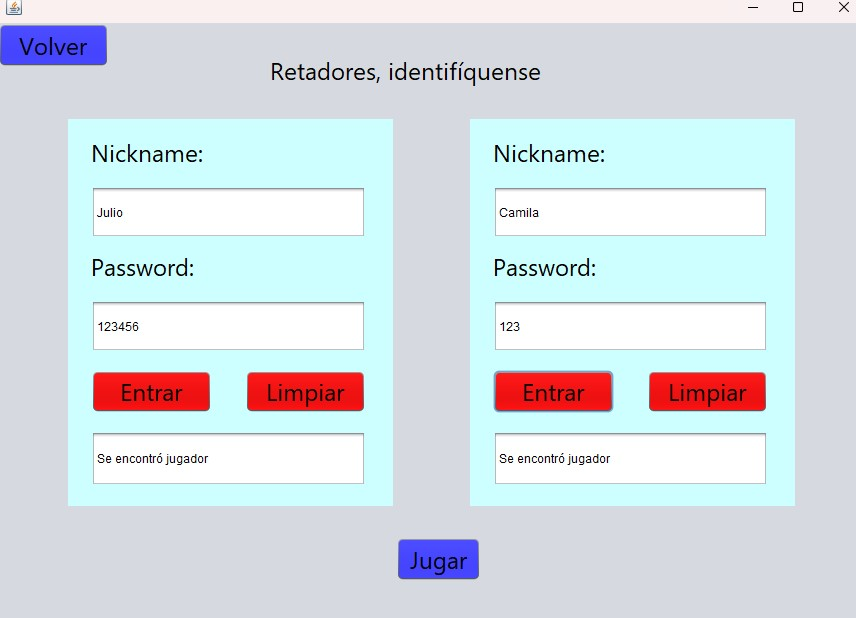
\includegraphics[width=1\textwidth,keepaspectratio]{img/entrar.jpg}
	%\includesvg{img/automata.svg}
	%\label{img:mot2}
	%\caption{Product backlog.}
\end{figure}

\begin{itemize}	
	\item Esta vendría a ser la ventana para poder ingresar a una partida con su usuario y contraseña, el botón jugar nos dirige al menú para seleccionar el reino y la arena
\end{itemize}

	
	
	
	

	\begin{lstlisting}[language=bash,caption={Commit: 2f725690a798849fc409e205c4096bf66af3cc1d }][H]
		git add .
		git commit -m "Se implementa las funcionalidades de crear ejercito y seleccionar arena en la clase QuickGameWindows"			
		git push -u origin main
	\end{lstlisting}
	
	
	\begin{itemize}
	\item Se opta por generar los ejércitos en esta ventana aprovechando que también se seleccionará el reino y la arena. Para evitar que el usuario apriete el botón "Generar Ejército" a cada rato, se decide que cuando el botón sea clickeado, se verifiquen una serie de cosas, como que se hayan seleccionado las arenas y los reinos,cuando ya se tiene esa información el botón cambie de valor a false (esto se logra con un método de la clase JButton) por lo que ahora ya no podrá ser clickeado. También se hace una serie de filtros en el Botón jugar que verifica que el valor del botón sea false. Para ambos casos, si no se logran cumplir las condiciones se lanza un mensaje de advertencia.
	\end{itemize}


		\begin{figure}[H]
		\centering
		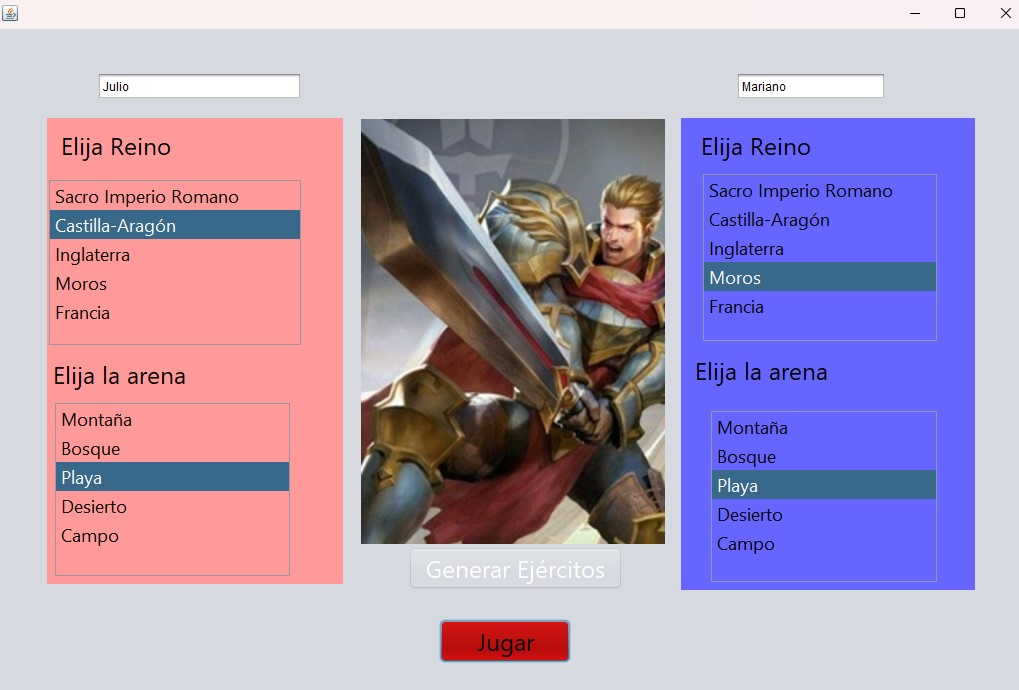
\includegraphics[width=1\textwidth,keepaspectratio]{img/optionsGame.jpg}
		%\includesvg{img/automata.svg}
		%\label{img:mot2}
		%\caption{Product backlog.}
	\end{figure}
	
	\begin{itemize}	
		\item Como podemos ver, se han seleccionado los reinos y las arenas, aparte de que se pulsó el botón "Generar Ejércitos", por lo que cambio el color.
	\end{itemize}
















	\begin{lstlisting}[language=bash,caption={Commit: b0ebb059321682a27d2f21c912ae36be7d544d08 }][H]
		git add .
		git commit -m "Se crea la clase jugar y se copia los metodos de la clase Aplicacion modifcandolo en lago, pero el juego se congela"			
		git push -u origin main
	\end{lstlisting}
	
	\begin{itemize}
	\item Ahora como ya se tenía la relación entre las ventanas, falta lo más importante, que era poder mover las piezas, o en otras palabras, poder empezar a jugar, para ello se copió los métodos que generaban el juego de la clase Aplicación a una nueva clase la cual se llama Juego, cuando se hizo la prueha, fue grande la sorpresa al ver que la ventana de había congelado
	\end{itemize}









	
	\begin{lstlisting}[language=bash,caption={Commit: 1026560a06a7659c2d6af35188a74a8c46d75c44 }][H]
		git add .
		git commit -m "Se soluciona el problema del tablero congelado"			
		git push -u origin main
	\end{lstlisting}
	
	
	\begin{itemize}
	\item Debido a una sobrecarga de la ventana, ya que se ejecutaban bucles y demás procesos, se decide hacer uso de hilos, para ser más específicos SwingWorker. Para evitar que el programa se congele, se crea una instancia de PrincipalFrame que representa la ventana principal del juego. Esta instancia se crea en el hilo de fondo (doInBackground) para evitar bloquear la interfaz de usuario durante la creación. 
	\end{itemize}


	\begin{lstlisting}[language=bash,caption={Commit: 3e51aab60d8dfbb00b2b5d27c9e9d890677624a5 }][H]
		git add .
		git commit -m "Se implementa la funcion de registro de victorias"			
		git push -u origin main
	\end{lstlisting}
	
	
	\begin{itemize}
		\item En el métodO game de la clase Jugar, después de que el método jugarTurnos culminé dictaminando un ganador, se implementa una serie de condiciones para poder determinar al ganador para que su victoria se sume a historial, esto a manea de darle uso a la base de datos, .
	\end{itemize}
	
	
	
	
	\begin{lstlisting}[language=bash,caption={Commit: c3f9cabe03aa0fe30794dc4f15b4fe910aa38ab2 }][H]
		git add .
		git commit -m "Se borra una clase y se termina de dar diminutas funcionalidades a las clases"			
		git push -u origin main
	\end{lstlisting}
	
	
	\begin{itemize}
		\item Más antes se habían realizado cambios, este commit más que nada evidencia los cambios que se hicieron, entre lo más rescatable se tiene la implementación de la función para mostrar jugadores, además de agregar una barra de menú con las opciones de poder guardar, ir a home y salir de la aplicación  
	\end{itemize}
	
			\begin{figure}[H]
		\centering
		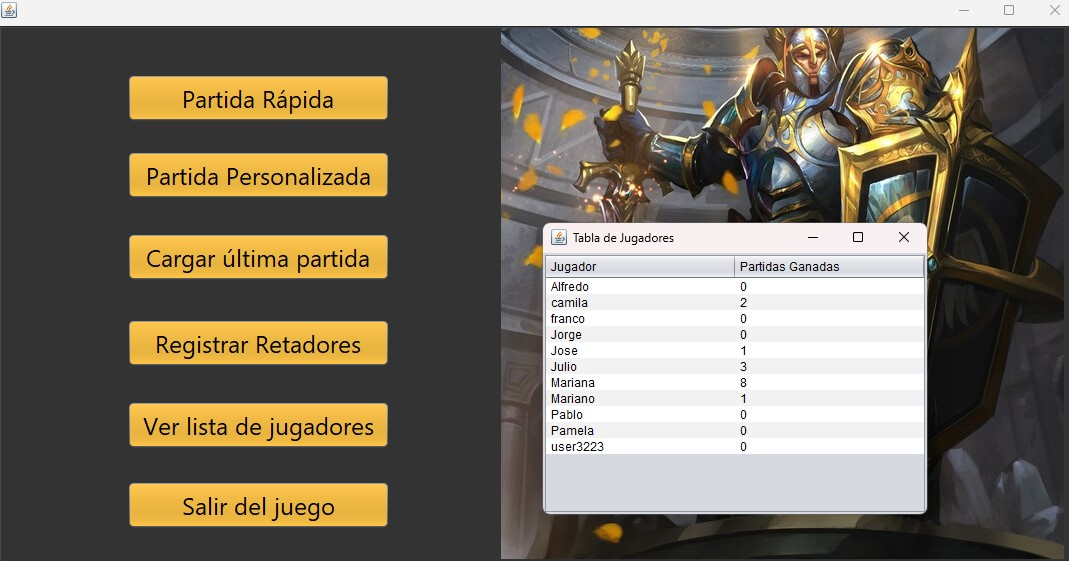
\includegraphics[width=1\textwidth,keepaspectratio]{img/historial.jpg}
		%\includesvg{img/automata.svg}
		%\label{img:mot2}
		%\caption{Product backlog.}
	\end{figure}
	
	\begin{itemize}	
		\item Como podemos ver, se han seleccionado los reinos y las arenas, aparte de que se pulsó el botón "Generar Ejércitos", por lo que cambio el color.
	\end{itemize}
	
	
	
	
	\begin{lstlisting}[language=bash,caption={Commit: 89ff6b1edf4542deb3ff42f005f490882c63ed89 }][H]
		git add .
		git commit -m "Se recupera la version anterior y se hace los cambios en las clases para poder implementar guardar, ahora falta hacer la consulta a la base de datos"			
		git push -u origin main
	\end{lstlisting}
	
	\begin{itemize}	
		\item Como nos falta crear la opción de cargar partida se decide crear la clase Partida la cual tendrá los atributos necesarios para reanudar el juego.
	\end{itemize}
	
	
	
	
		\begin{lstlisting}[language=bash,caption={Commit: e24b6eb460d4e868fad82818e2b735efea714c23 }][H]
		git add .
		git commit -m "Se crea el metodo guardarPartida"			
		git push -u origin main
	\end{lstlisting}
	
	\begin{itemize}	
		\item En la clase Conectar se implementa la lógica y la clase PrincipalFrame la llama cuando se da click al botón guardar.
	\end{itemize}
	
	
			\begin{lstlisting}[language=bash,caption={Commit: c15b7d87562a4a723111d504c4ae5b4a27526f91 }][H]
		git add .
		git commit -m "Se crea la opcion de cargar partida"			
		git push -u origin main
	\end{lstlisting}
	
	\begin{itemize}	
		\item En la clase HomeGame se implementa la acción de poder cargar la última partida.
	\end{itemize}
	
	
	
	\begin{lstlisting}[language=bash,caption={Interfaz del juego}][H]
		javac HomeGame.java
		java HomeGame
	\end{lstlisting}

	\begin{figure}[H]
		\centering
		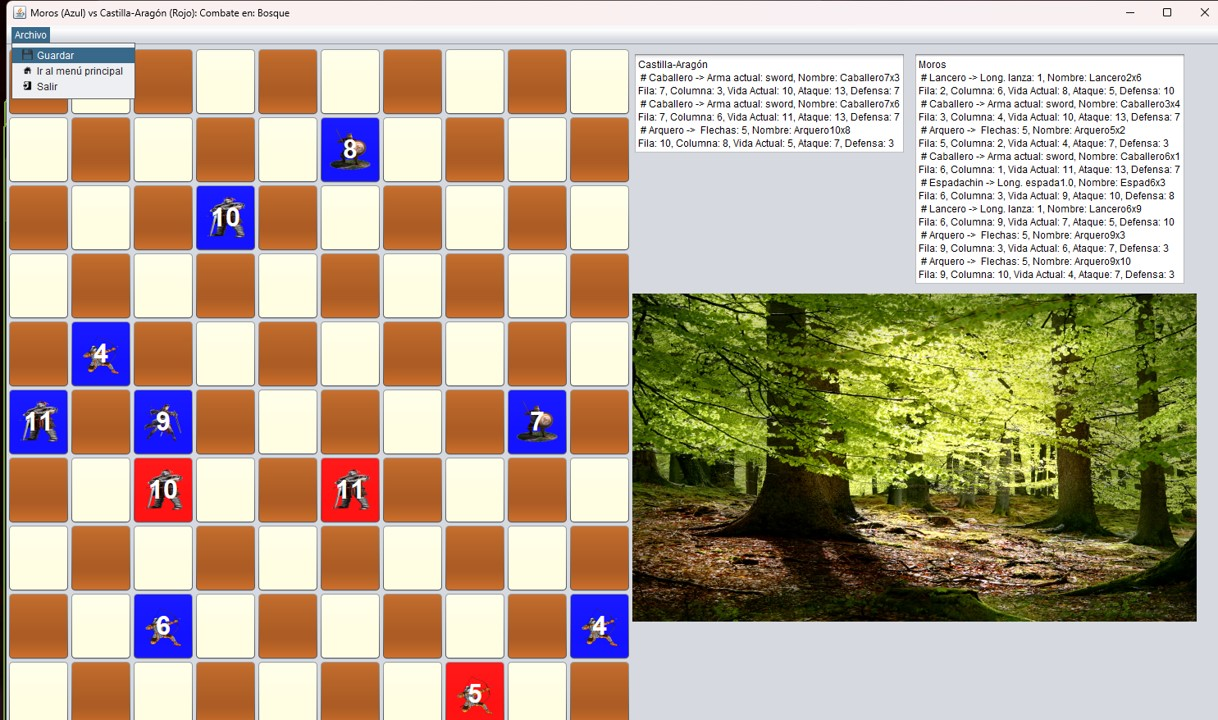
\includegraphics[width=1\textwidth,keepaspectratio]{img/test.jpg}
		%\includesvg{img/automata.svg}
		%\label{img:mot2}
		%\caption{Product backlog.}
	\end{figure}
	
	\begin{itemize}	
		\item Se puede apreciar la ejecución del juego, además de que en la parte superior de la izquierda se puede apreciar un pequeño menú, debido al tiempo la función de guardar no se encuentra disponible, pero si las demás
	\end{itemize}
	
	
	
	
	
	\lstinputlisting[language=Java, caption={Jugar.java},numbers=left,]{src/Jugar.java}
	
	\begin{itemize}	
		\item El enfoque de usar hilos hace posible que las fichas puedan moverse, ya que si no se hubiera usado SwingWorker la ventana se congelaría 
	\end{itemize}
	
	
	
	\subsection{Diagrama UML}
	
	\begin{figure}[H]
		\centering
		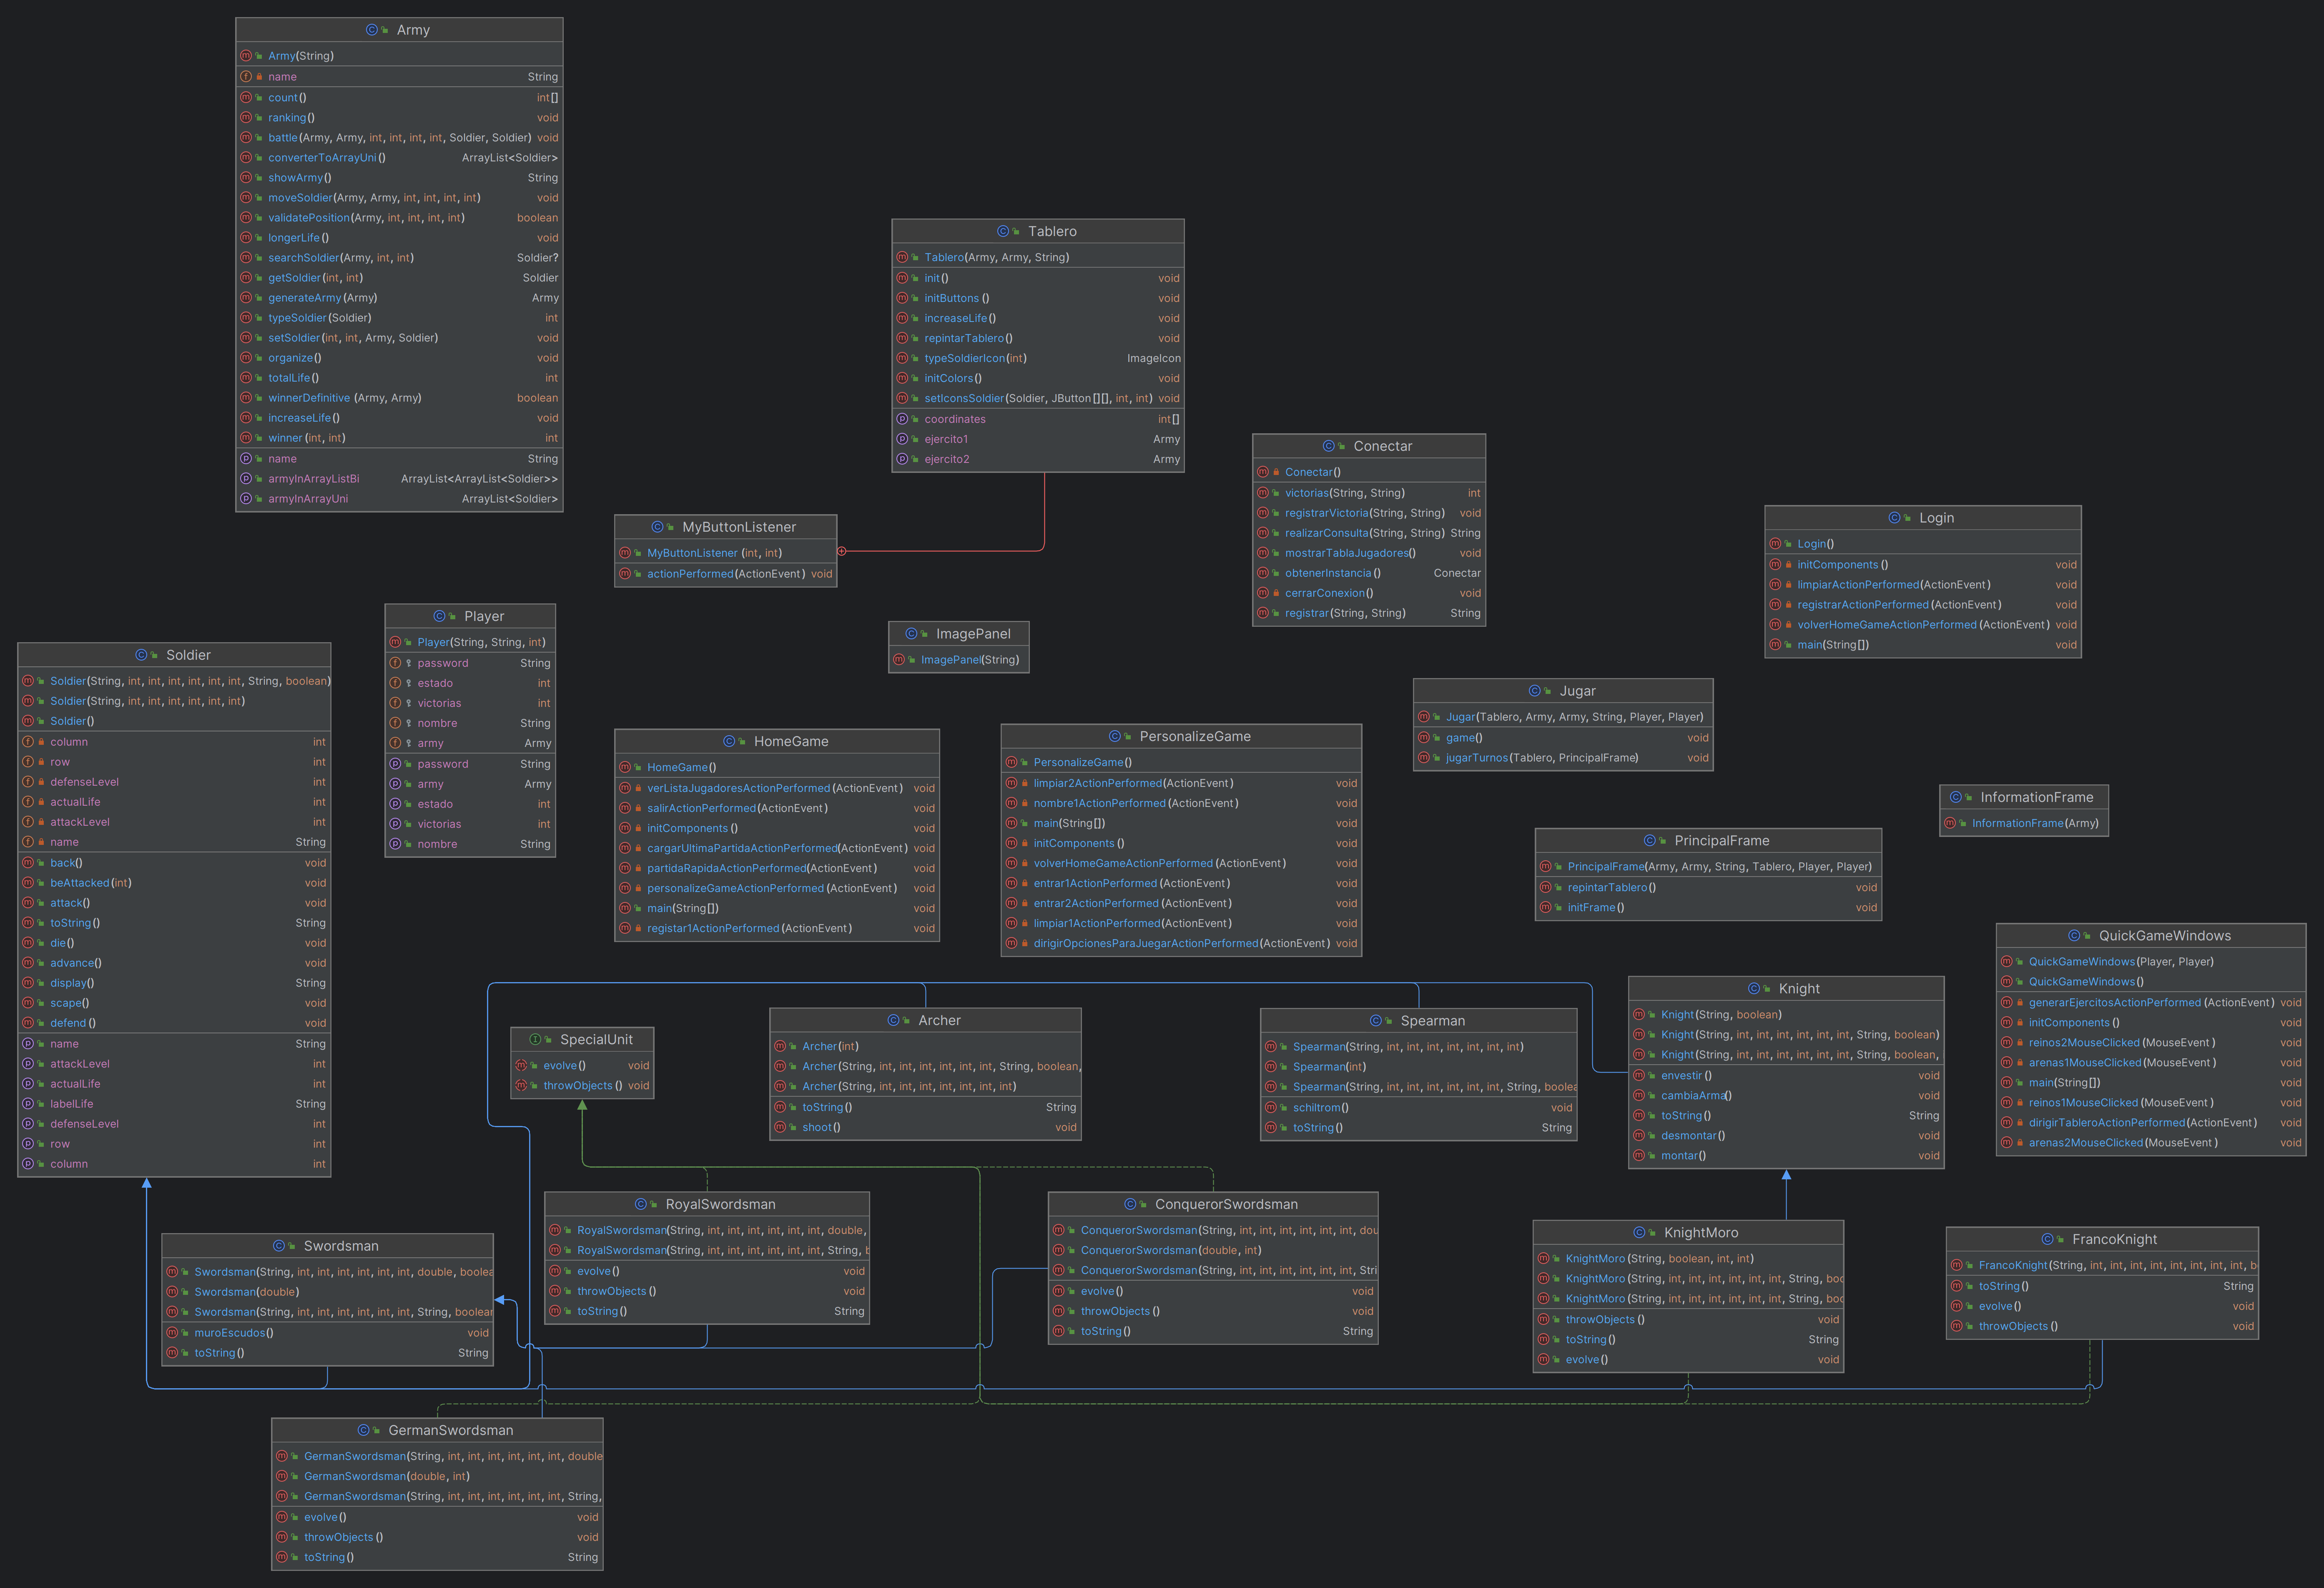
\includegraphics[width=1\textwidth,keepaspectratio]{img/uml.png}
		%\includesvg{img/automata.svg}
		%\label{img:mot2}
		%\caption{Product backlog.}
	\end{figure}
	
	\begin{itemize}	
			\item Si hay problemas en la visualización, puede ver la imagen en la carpeta img (descárgela)
	\end{itemize}
	
	
	
	
	
	\subsection{Estructura de laboratorio 23}
	\begin{itemize}	
		\item El contenido que se entrega en este laboratorio es el siguiente:
	\end{itemize}
	


	\begin{figure}[H]
		\centering
		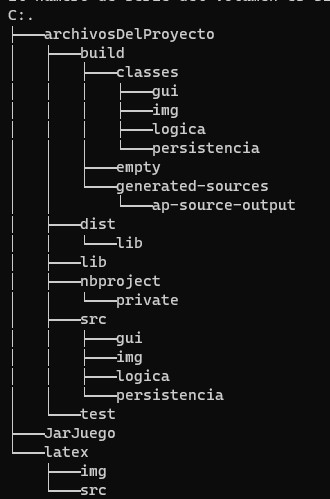
\includegraphics[width=0.6\textwidth,keepaspectratio]{img/tree.jpg}
		%\includesvg{img/automata.svg}
		%\label{img:mot2}
		%\caption{Product backlog.}
	\end{figure}	
	
	\begin{itemize}	
		\item Debido a problemas en la codificación de latex con ciertos caracteres que genera el comando tree f, se opta 
		por enviar la estructura de este laboratorio en formato de imagen
	\end{itemize}
	

   
	
	\section{\textcolor{red}{Rúbricas}}
	
	\subsection{\textcolor{red}{Entregable Informe}}
	\begin{table}[H]
		\caption{Tipo de Informe}
		\setlength{\tabcolsep}{0.5em} % for the horizontal padding
		{\renewcommand{\arraystretch}{1.5}% for the vertical padding
			\begin{tabular}{|p{3cm}|p{12cm}|}
				\hline
				\multicolumn{2}{|c|}{\textbf{\textcolor{red}{Informe}}}  \\
				\hline 
				\textbf{\textcolor{red}{Latex}} & \textcolor{blue}{El informe está en formato PDF desde Latex,  con un formato limpio (buena presentación) y facil de leer.}   \\ 
				\hline 
				
				
			\end{tabular}
		}
	\end{table}
	
	\clearpage
	
	\subsection{\textcolor{red}{Rúbrica para el contenido del Informe y demostración}}
	\begin{itemize}			
		\item El alumno debe marcar o dejar en blanco en celdas de la columna \textbf{Checklist} si cumplio con el ítem correspondiente.
		\item Si un alumno supera la fecha de entrega,  su calificación será sobre la nota mínima aprobada, siempre y cuando cumpla con todos lo items.
		\item El alumno debe autocalificarse en la columna \textbf{Estudiante} de acuerdo a la siguiente tabla:
		
		\begin{table}[ht]
			\caption{Niveles de desempeño}
			\begin{center}
				\begin{tabular}{ccccc}
					\hline
					& \multicolumn{4}{c}{Nivel}\\
					\cline{1-5}
					\textbf{Puntos} & Insatisfactorio 25\%& En Proceso 50\% & Satisfactorio 75\% & Sobresaliente 100\%\\
					\textbf{2.0}&0.5&1.0&1.5&2.0\\
					\textbf{4.0}&1.0&2.0&3.0&4.0\\
					\hline
				\end{tabular}
			\end{center}
		\end{table}	
		
	\end{itemize}
	
	\begin{table}[H]
		\caption{Rúbrica para contenido del Informe y demostración}
		\setlength{\tabcolsep}{0.5em} % for the horizontal padding
		{\renewcommand{\arraystretch}{1.5}% for the vertical padding
			%\begin{center}
			\begin{tabular}{|p{2.7cm}|p{7cm}|x{1.3cm}|p{1.2cm}|p{1.5cm}|p{1.1cm}|}
				\hline
				\multicolumn{2}{|c|}{Contenido y demostración} & Puntos & Checklist & Estudiante & Profesor\\
				\hline
				\textbf{1. GitHub} & Hay enlace URL activo del directorio para el  laboratorio hacia su repositorio GitHub con código fuente terminado y fácil de revisar. &2 &X &2 & \\ 
				\hline
				\textbf{2. Commits} &  Hay capturas de pantalla de los commits más importantes con sus explicaciones detalladas. (El profesor puede preguntar para refrendar calificación). &4 &X &4 & \\ 
				\hline 
				\textbf{3. Código fuente} &  Hay porciones de código fuente importantes con numeración y explicaciones detalladas de sus funciones. &2 &X &2 & \\ 
				\hline 
				\textbf{4. Ejecución} & Se incluyen ejecuciones/pruebas del código fuente  explicadas gradualmente. &2 &X &2 & \\ 
				\hline			
				\textbf{5. Pregunta} & Se responde con completitud a la pregunta formulada en la tarea.  (El profesor puede preguntar para refrendar calificación).  &2 &X &2 & \\ 
				\hline	
				\textbf{6. Fechas} & Las fechas de modificación del código fuente estan dentro de los plazos de fecha de entrega establecidos. &2 &X &2 & \\ 
				\hline 
				\textbf{7. Ortografía} & El documento no muestra errores ortográficos. &2 &X &2 & \\ 
				\hline 
				\textbf{8. Madurez} & El Informe muestra de manera general una evolución de la madurez del código fuente,  explicaciones puntuales pero precisas y un acabado impecable.   (El profesor puede preguntar para refrendar calificación).  &4 &X &2 & \\ 
				\hline
				\multicolumn{2}{|c|}{\textbf{Total}} &20 & &18 & \\ 
				\hline
			\end{tabular}
			%\end{center}
			%\label{tab:multicol}
		}
	\end{table}
	
	\clearpage
	
	\section{Referencias}
	\begin{itemize}			
		\item \url{https://www.geeksforgeeks.org/insertion-sort/}
	\end{itemize}	
	
	%\clearpage
	%\bibliographystyle{apalike}
	%\bibliographystyle{IEEEtranN}
	%\bibliography{bibliography}
	
\end{document}